\thispagestyle{plain}
\section{Mean values and variance}\label{sec:appendix_a}
%
\noindent The main regression method used in this report is the ordinary least squares method.
This appensix shows the calculations for some of the equations used to produce the results shown in this report.
%
We have assumed that our data can be described by the continous function 
$f(\boldsymbol{x})$, and an error term $\boldsymbol{\epsilon} ~ N(0, \sigma^{2})$. 
If we approximate the function with the solution derived from a model $\boldsymbol{\tilde{y}} = X\boldsymbol{\beta}$ the data can be described with $\boldsymbol{y} = X\boldsymbol{\beta} + \boldsymbol{\epsilon}$. 
The expectation value 
%
\begin{align*}
    %\hskip\parindent
    \mathbb{E}(\boldsymbol{y}) &= \mathbb{E}(X\boldsymbol{\beta} + \boldsymbol{\epsilon}) \\
    &= \mathbb{E}(X\boldsymbol{\beta}) + \mathbb{E}(\boldsymbol{\epsilon}) && \text{where the expected value $\boldsymbol{\epsilon} = 0$} \\
    \mathbb{E}(y_{i}) &= \sum_{j=0}^{P-1} X_{i,j} \beta_{j} && \text{for the each element} \\
    &= X_{i,*} \beta_{i} && \text{where $_{*}$ replace the sum over index $i$} \\
\end{align*}
%
The variance for the element $y_{i}$ can be found by
\begin{align*}
    \mathbb{V}(y_{i}) &= \mathbb{E} \big[ (y_{i} - \mathbb{E}(y_{i}))^{2} \big] \\
    &= \mathbb{E} (y_{i}^{2}) - (\mathbb{E}(y_{i})^{2}) \\
    &= \mathbb{E} ((X_{i,*} \beta_{i} + \epsilon_{i})^{2}) - (X_{i,*} \beta_{i})^{2} \\
    &= \mathbb{E} ((X_{i,*} \beta_{i})^{2} + 2\epsilon_{i}X_{i,*} \beta_{i} + \epsilon^{2}) - (X_{i,*} \beta_{i})^{2} \\
    &= \mathbb{E} ((X_{i,*} \beta_{i})^{2}) + \mathbb{E} (2\epsilon_{i}X_{i,*} \beta_{i}) + \mathbb{E} (\epsilon^{2}) - (X_{i,*} \beta_{i})^{2} \\
    &= (X_{i,*} \beta_{i})^{2} + \mathbb{E} (\epsilon^{2}) - (X_{i,*} \beta_{i})^{2} \\
    &= \mathbb{E} (\epsilon^{2}) = \sigma^{2} \\
\end{align*}
%
The expression for the optimal parameter 
\begin{align*}
    \boldsymbol{\hat{\beta}} &= (\boldsymbol{X}^{T} \boldsymbol{X})^{-1} \boldsymbol{X}^{T} \boldsymbol{y} \\
\end{align*}
We find the expected value of $\boldsymbol{\hat{\beta}}$
\begin{align*}
    \mathbb{E}(\boldsymbol{\hat{\beta}}) &= \mathbb{E}((\boldsymbol{X}^{T} \boldsymbol{X})^{-1} \boldsymbol{X}^{T} \boldsymbol{y}) \\
    &= (\boldsymbol{X}^{T} \boldsymbol{X})^{-1} \boldsymbol{X}^{T} \mathbb{E}(\boldsymbol{y}) && \text{using that $\boldsymbol{X}$ is a non-stochastic variable} \\
    &= (\boldsymbol{X}^{T} \boldsymbol{X})^{-1} \boldsymbol{X}^{T} \boldsymbol{X} \boldsymbol{\beta} && \text{using $\mathbb{E}(\boldsymbol{y}) = \boldsymbol{X} \boldsymbol{\beta}$} \\
    &= \boldsymbol{\beta} \\
\end{align*}
%
We can find the variance by 
\begin{align*}
    \mathbb{V}(\boldsymbol{\hat{\beta}}) &= \mathbb{E} \big[ (\boldsymbol{\hat{\beta}} - \mathbb{E}(\boldsymbol{\hat{\beta}}))^{2} \big] \\
    &= \mathbb{E} (\boldsymbol{\hat{\beta}} \boldsymbol{\hat{\beta}}^{T}) - \mathbb{E}(\boldsymbol{\hat{\beta}})^{2}  \\
    &= \mathbb{E} (((\boldsymbol{X}^{T} \boldsymbol{X})^{-1} \boldsymbol{X}^{T} \boldsymbol{y}) ((\boldsymbol{X}^{T} \boldsymbol{X})^{-1} \boldsymbol{X}^{T} \boldsymbol{y})^{T}) - \boldsymbol{\hat{\beta}}\boldsymbol{\hat{\beta}}^{T}  \\
    &= \mathbb{E} ((\boldsymbol{X}^{T} \boldsymbol{X})^{-1} \boldsymbol{X}^{T} \boldsymbol{y} \boldsymbol{y}^{T} \boldsymbol{X} (\boldsymbol{X}^{T} \boldsymbol{X})^{-1}) - \boldsymbol{\hat{\beta}}\boldsymbol{\hat{\beta}}^{T}  \\
    &= (\boldsymbol{X}^{T} \boldsymbol{X})^{-1} \boldsymbol{X}^{T} \mathbb{E} (\boldsymbol{y} \boldsymbol{y}^{T}) \boldsymbol{X} (\boldsymbol{X}^{T} \boldsymbol{X})^{-1} - \boldsymbol{\hat{\beta}}\boldsymbol{\hat{\beta}}^{T}  \\
    &= (\boldsymbol{X}^{T} \boldsymbol{X})^{-1} \boldsymbol{X}^{T} (\boldsymbol{X} \boldsymbol{\beta} \boldsymbol{\beta}^{T} \boldsymbol{X}^{T} + \sigma^{2}) \boldsymbol{X} (\boldsymbol{X}^{T} \boldsymbol{X})^{-1} - \boldsymbol{\hat{\beta}}\boldsymbol{\hat{\beta}}^{T}  \\
    &= \boldsymbol{\beta} \boldsymbol{\beta}^{T} + \sigma^{2}((\boldsymbol{X}^{T} \boldsymbol{X})^{-1} \boldsymbol{X}^{T} \boldsymbol{X} (\boldsymbol{X}^{T} \boldsymbol{X})^{-1}) - \boldsymbol{\hat{\beta}}\boldsymbol{\hat{\beta}}^{T}  \\
    &= \sigma^{2}(\boldsymbol{X}^{T} \boldsymbol{X})^{-1} \\
\end{align*}
Knowing the expectation value and the variance of $\boldsymbol{\hat{\beta}}$, we can define a confidence interval for each $\hat{\beta}_{j} \pm std(\hat{\beta}_j)$ for $j=1, 2, \hdots, P-1$.
%
The optimal $\boldsymbol{\hat{\beta}}^{Ridge}$ can be derived from MSE, and is defined as 
\begin{align*}
    \boldsymbol{\hat{\beta}}^{Ridge} &= (\boldsymbol{X}^{T}\boldsymbol{X} + \lambda \boldsymbol{I})^{-1} \boldsymbol{X}^{T} \boldsymbol{y} \\
\end{align*}
The expectation value is then 
\begin{align*}
    \mathbb{E} (\boldsymbol{\hat{\beta}}^{Ridge}) &= \mathbb{E}((\boldsymbol{X}^{T}\boldsymbol{X} + \lambda \boldsymbol{I})^{-1} \boldsymbol{X}^{T} \boldsymbol{y}) \\
    &= (\boldsymbol{X}^{T}\boldsymbol{X} + \lambda \boldsymbol{I})^{-1} \boldsymbol{X}^{T} \mathbb{E}( \boldsymbol{y} ) && \text{since $\boldsymbol{X}$ and $\lambda \boldsymbol{I}$ are non-stochastic variables} \\
    &= (\boldsymbol{X}^{T}\boldsymbol{X} + \lambda \boldsymbol{I})^{-1} \boldsymbol{X}^{T} \boldsymbol{X} \boldsymbol{\beta} && \text{using $\mathbb{E} (\boldsymbol{y})$ from exercise 1} \\
\end{align*}
For $\lambda = 0$ we have $\mathbb{E} (\boldsymbol{\hat{\beta}}^{OLS})$. The variance 
\begin{align*}
    \mathbb{V}(\boldsymbol{\hat{\beta}}^{Ridge}) &= \mathbb{E} (\boldsymbol{\hat{\beta}}_{R} \boldsymbol{\hat{\beta}}_{R}^{T}) - (\mathbb{E} (\boldsymbol{\hat{\beta}}_{R}))^{2} \\
    &= \mathbb{E} (((\boldsymbol{X}^{T}\boldsymbol{X} + \lambda \boldsymbol{I})^{-1} \boldsymbol{X}^{T} \boldsymbol{y}) (((\boldsymbol{X}^{T}\boldsymbol{X} + \lambda \boldsymbol{I})^{-1} \boldsymbol{X}^{T} \boldsymbol{y}))^{T}) - (\mathbb{E} (\boldsymbol{\hat{\beta}}_{R}))^{2} \\
    &= \mathbb{E} ((\boldsymbol{X}^{T}\boldsymbol{X} + \lambda \boldsymbol{I})^{-1} \boldsymbol{X}^{T} \boldsymbol{y} \boldsymbol{y}^{T} \boldsymbol{X} ((\boldsymbol{X}^{T}\boldsymbol{X} + \lambda \boldsymbol{I})^{-1})^{T} ) - (\mathbb{E} (\boldsymbol{\hat{\beta}}_{R}))^{2} \\
    &= (\boldsymbol{X}^{T}\boldsymbol{X} + \lambda \boldsymbol{I})^{-1} \boldsymbol{X}^{T} \mathbb{E} (\boldsymbol{y} \boldsymbol{y}^{T} ) \boldsymbol{X} ((\boldsymbol{X}^{T}\boldsymbol{X} + \lambda \boldsymbol{I})^{-1})^{T} - (\mathbb{E} (\boldsymbol{\hat{\beta}}_{R}))^{2} \\
    &= (\boldsymbol{X}^{T}\boldsymbol{X} + \lambda \boldsymbol{I})^{-1} \boldsymbol{X}^{T} (\boldsymbol{X} \boldsymbol{\beta} \boldsymbol{\beta}^{T} \boldsymbol{X}^{T} + \sigma^{2}) \boldsymbol{X} ((\boldsymbol{X}^{T}\boldsymbol{X} + \lambda \boldsymbol{I})^{-1})^{T} - (\mathbb{E} (\boldsymbol{\hat{\beta}}_{R}))^{2} \\
    &= \sigma^{2}(\boldsymbol{X}^{T}\boldsymbol{X} + \lambda \boldsymbol{I})^{-1} \boldsymbol{X}^{T} \boldsymbol{X} ((\boldsymbol{X}^{T}\boldsymbol{X} + \lambda \boldsymbol{I})^{-1})^{T} + (\mathbb{E} (\boldsymbol{\hat{\beta}}_{R}))^{2} - (\mathbb{E} (\boldsymbol{\hat{\beta}}_{R}))^{2} \\
    &= \sigma^{2}(\boldsymbol{X}^{T}\boldsymbol{X} + \lambda \boldsymbol{I})^{-1} \boldsymbol{X}^{T} \boldsymbol{X} ((\boldsymbol{X}^{T}\boldsymbol{X} + \lambda \boldsymbol{I})^{-1})^{T} \\
\end{align*}


\section{Bias-variance trade-off}\label{sec:appendix_b}
\noindent From equation $\boldsymbol{y} = f(\boldsymbol{x}) + \boldsymbol{\epsilon}$ and the assumption $f(\boldsymbol{x}) \approx \boldsymbol{\tilde{y}} = \boldsymbol{X \beta}$
The expectation value of the mean square error is 
\begin{align*}
	\mathbb{E}((\boldsymbol{y} - \boldsymbol{\tilde{y}})^{2}) &= \mathbb{E}(\boldsymbol{y}^{2}) - 2 \mathbb{E}(\boldsymbol{y} \boldsymbol{\tilde{y}}) \mathbb{E}(\boldsymbol{\tilde{y}}^{2}) \\
	&= \mathbb{E}(f(\boldsymbol{x})^{2}) + \mathbb{E}(\boldsymbol{\epsilon}^{2}) - 2 f(\boldsymbol{x}) \mathbb{E}(\boldsymbol{\tilde{y}}) + \mathbb{V}(\boldsymbol{\tilde{y}}) + \mathbb{E}(\boldsymbol{\tilde{y}})^{2} \\
	&= f(\boldsymbol{x})^{2} - 2 f(\boldsymbol{x}) \mathbb{E}(\boldsymbol{\tilde{y}}) + \mathbb{E}(\boldsymbol{\tilde{y}})^{2} + \mathbb{V}(\boldsymbol{\tilde{y}}) + \mathbb{V}(\boldsymbol{\epsilon}) \\
	&= \mathbb{E}((f(\boldsymbol{x}) - \mathbb{E}(\boldsymbol{\tilde{y}}))^{2}) + \mathbb{V}(\boldsymbol{\tilde{y}}) + \sigma^{2}
\end{align*}

\newpage
\section{Plots}\label{sec:appendix_c}
Here we have collected some interesting plots from the analysis of the Franke function and the terrain data :)
%
\subsection{Franke function}
\begin{figure}[H]
	\centering
	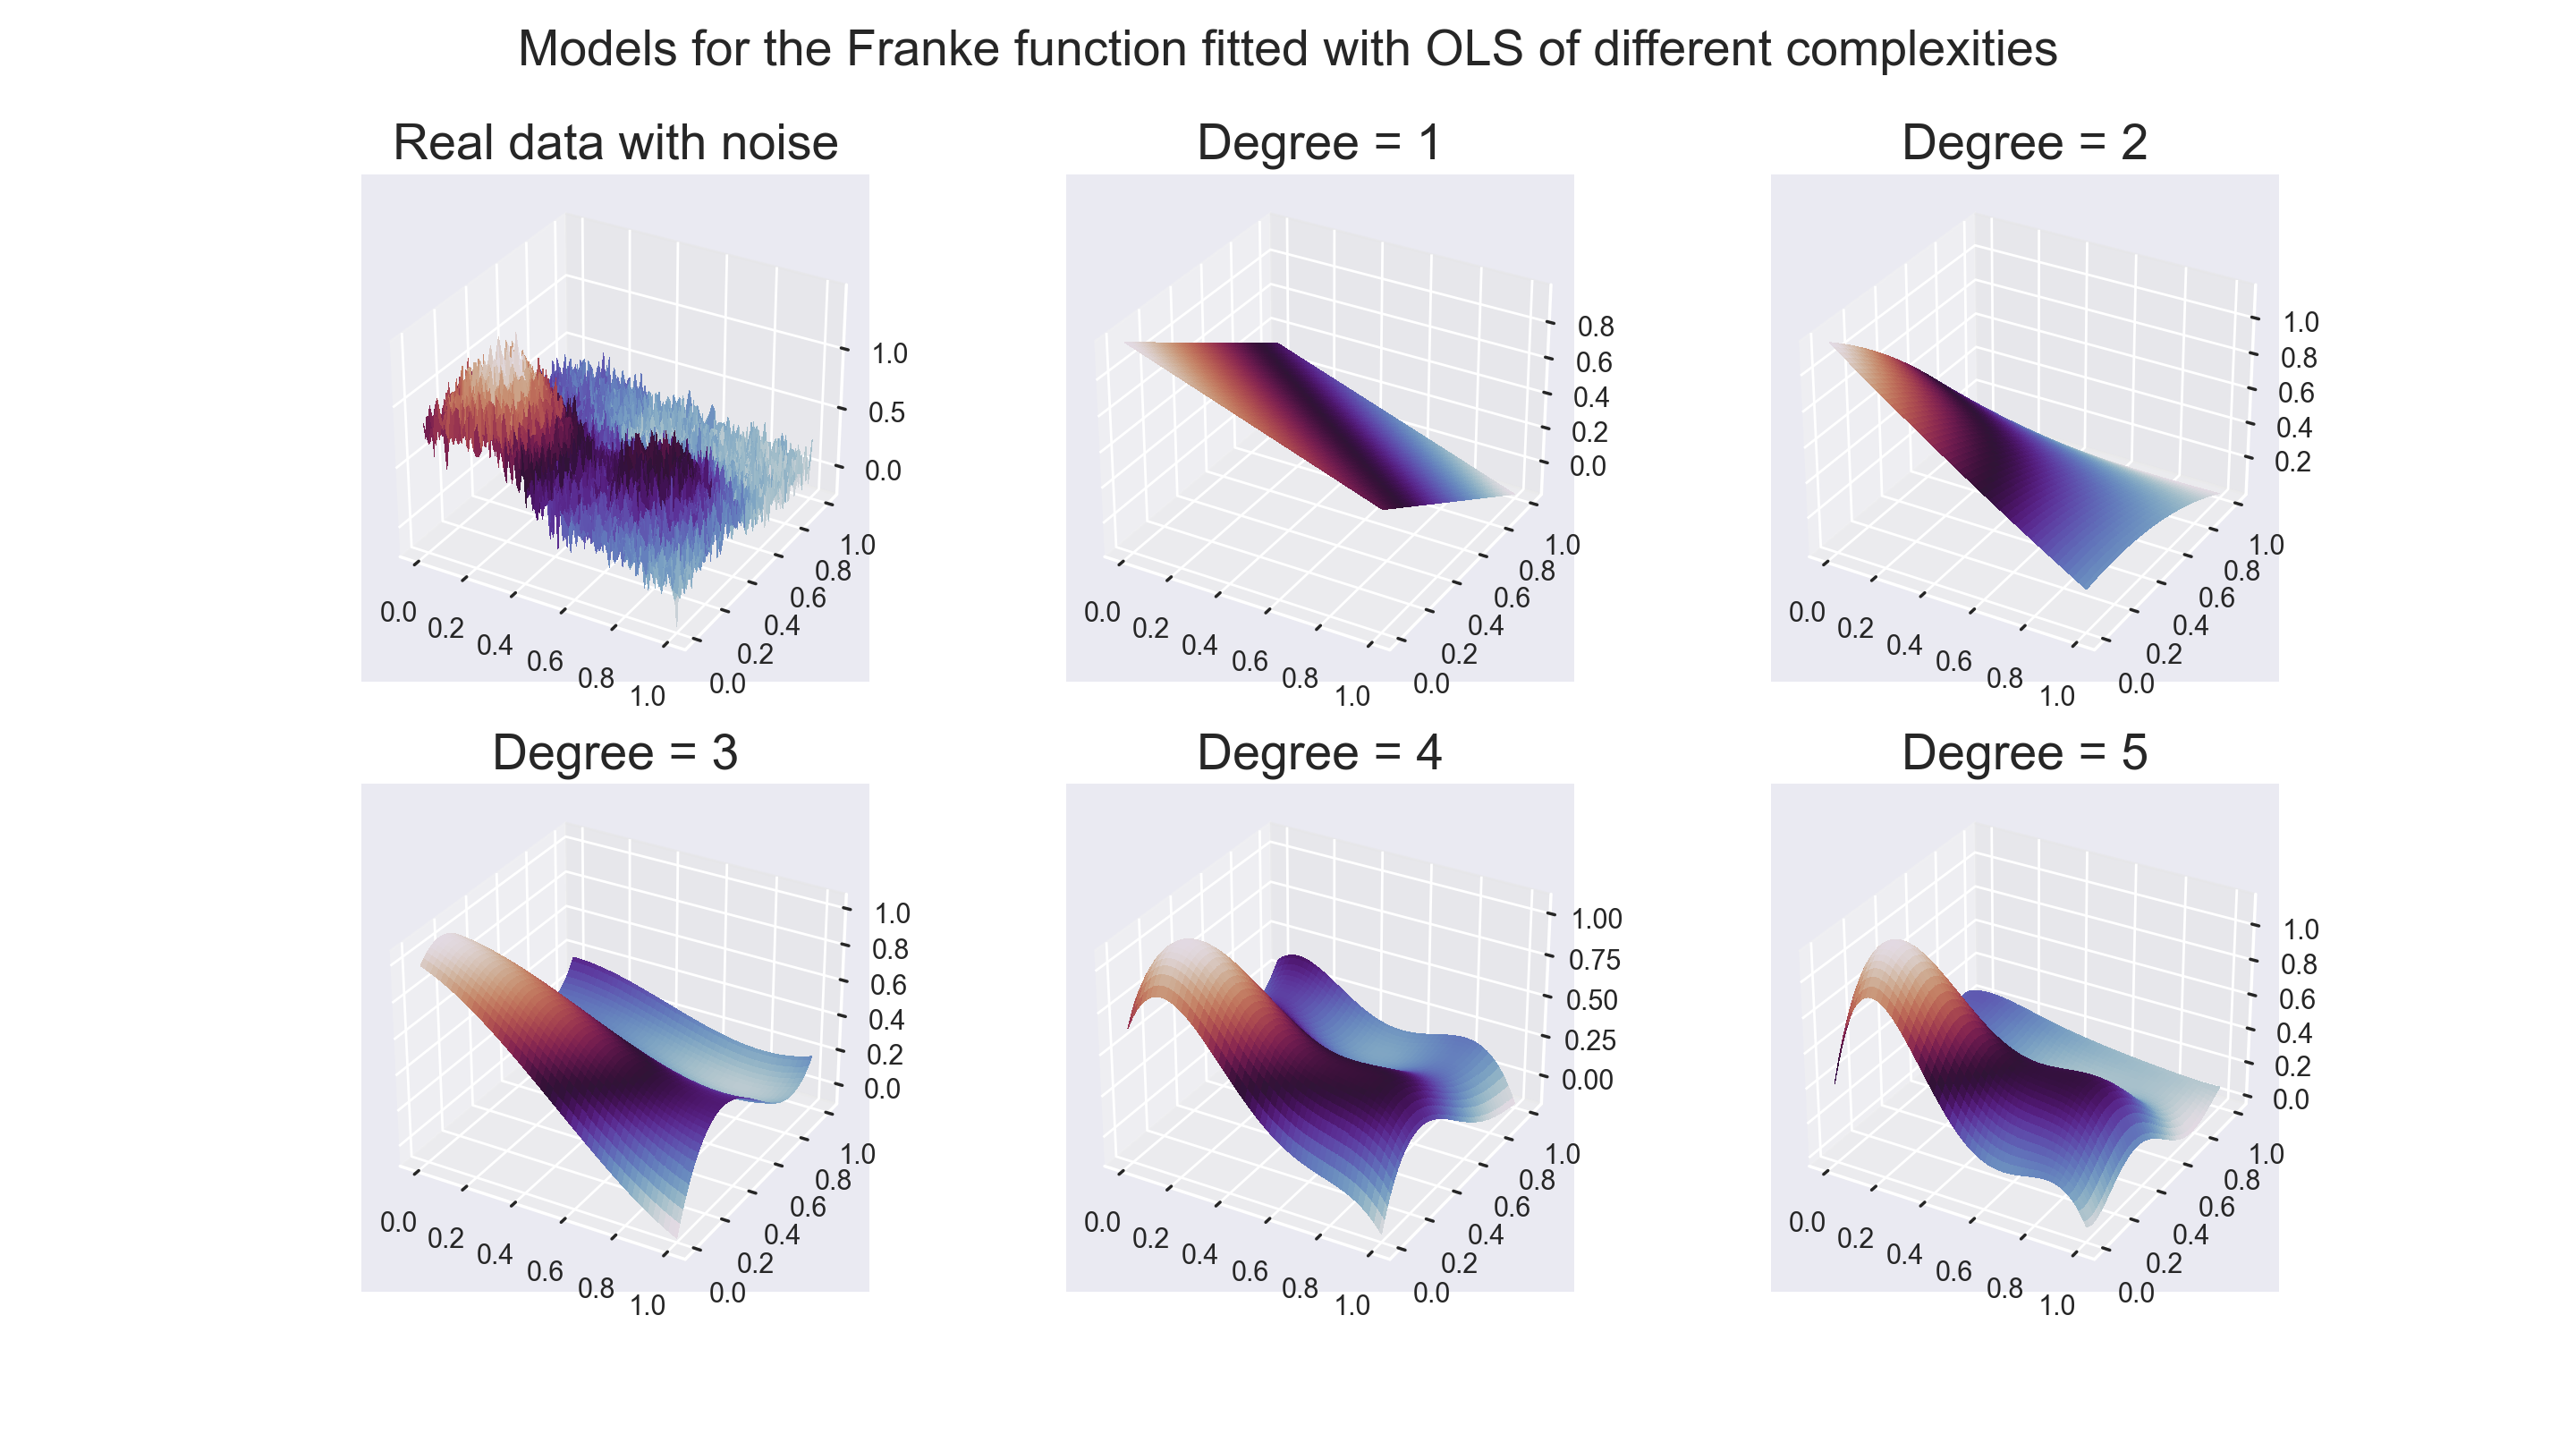
\includegraphics[width=\linewidth]{images/Figure_2.png}
	\caption{A plot showing how a model of different complexities fit the franke function when OLS regession has been used.}
	\label{OLS figure}
\end{figure}
%
\begin{figure}[H]
	\centering
	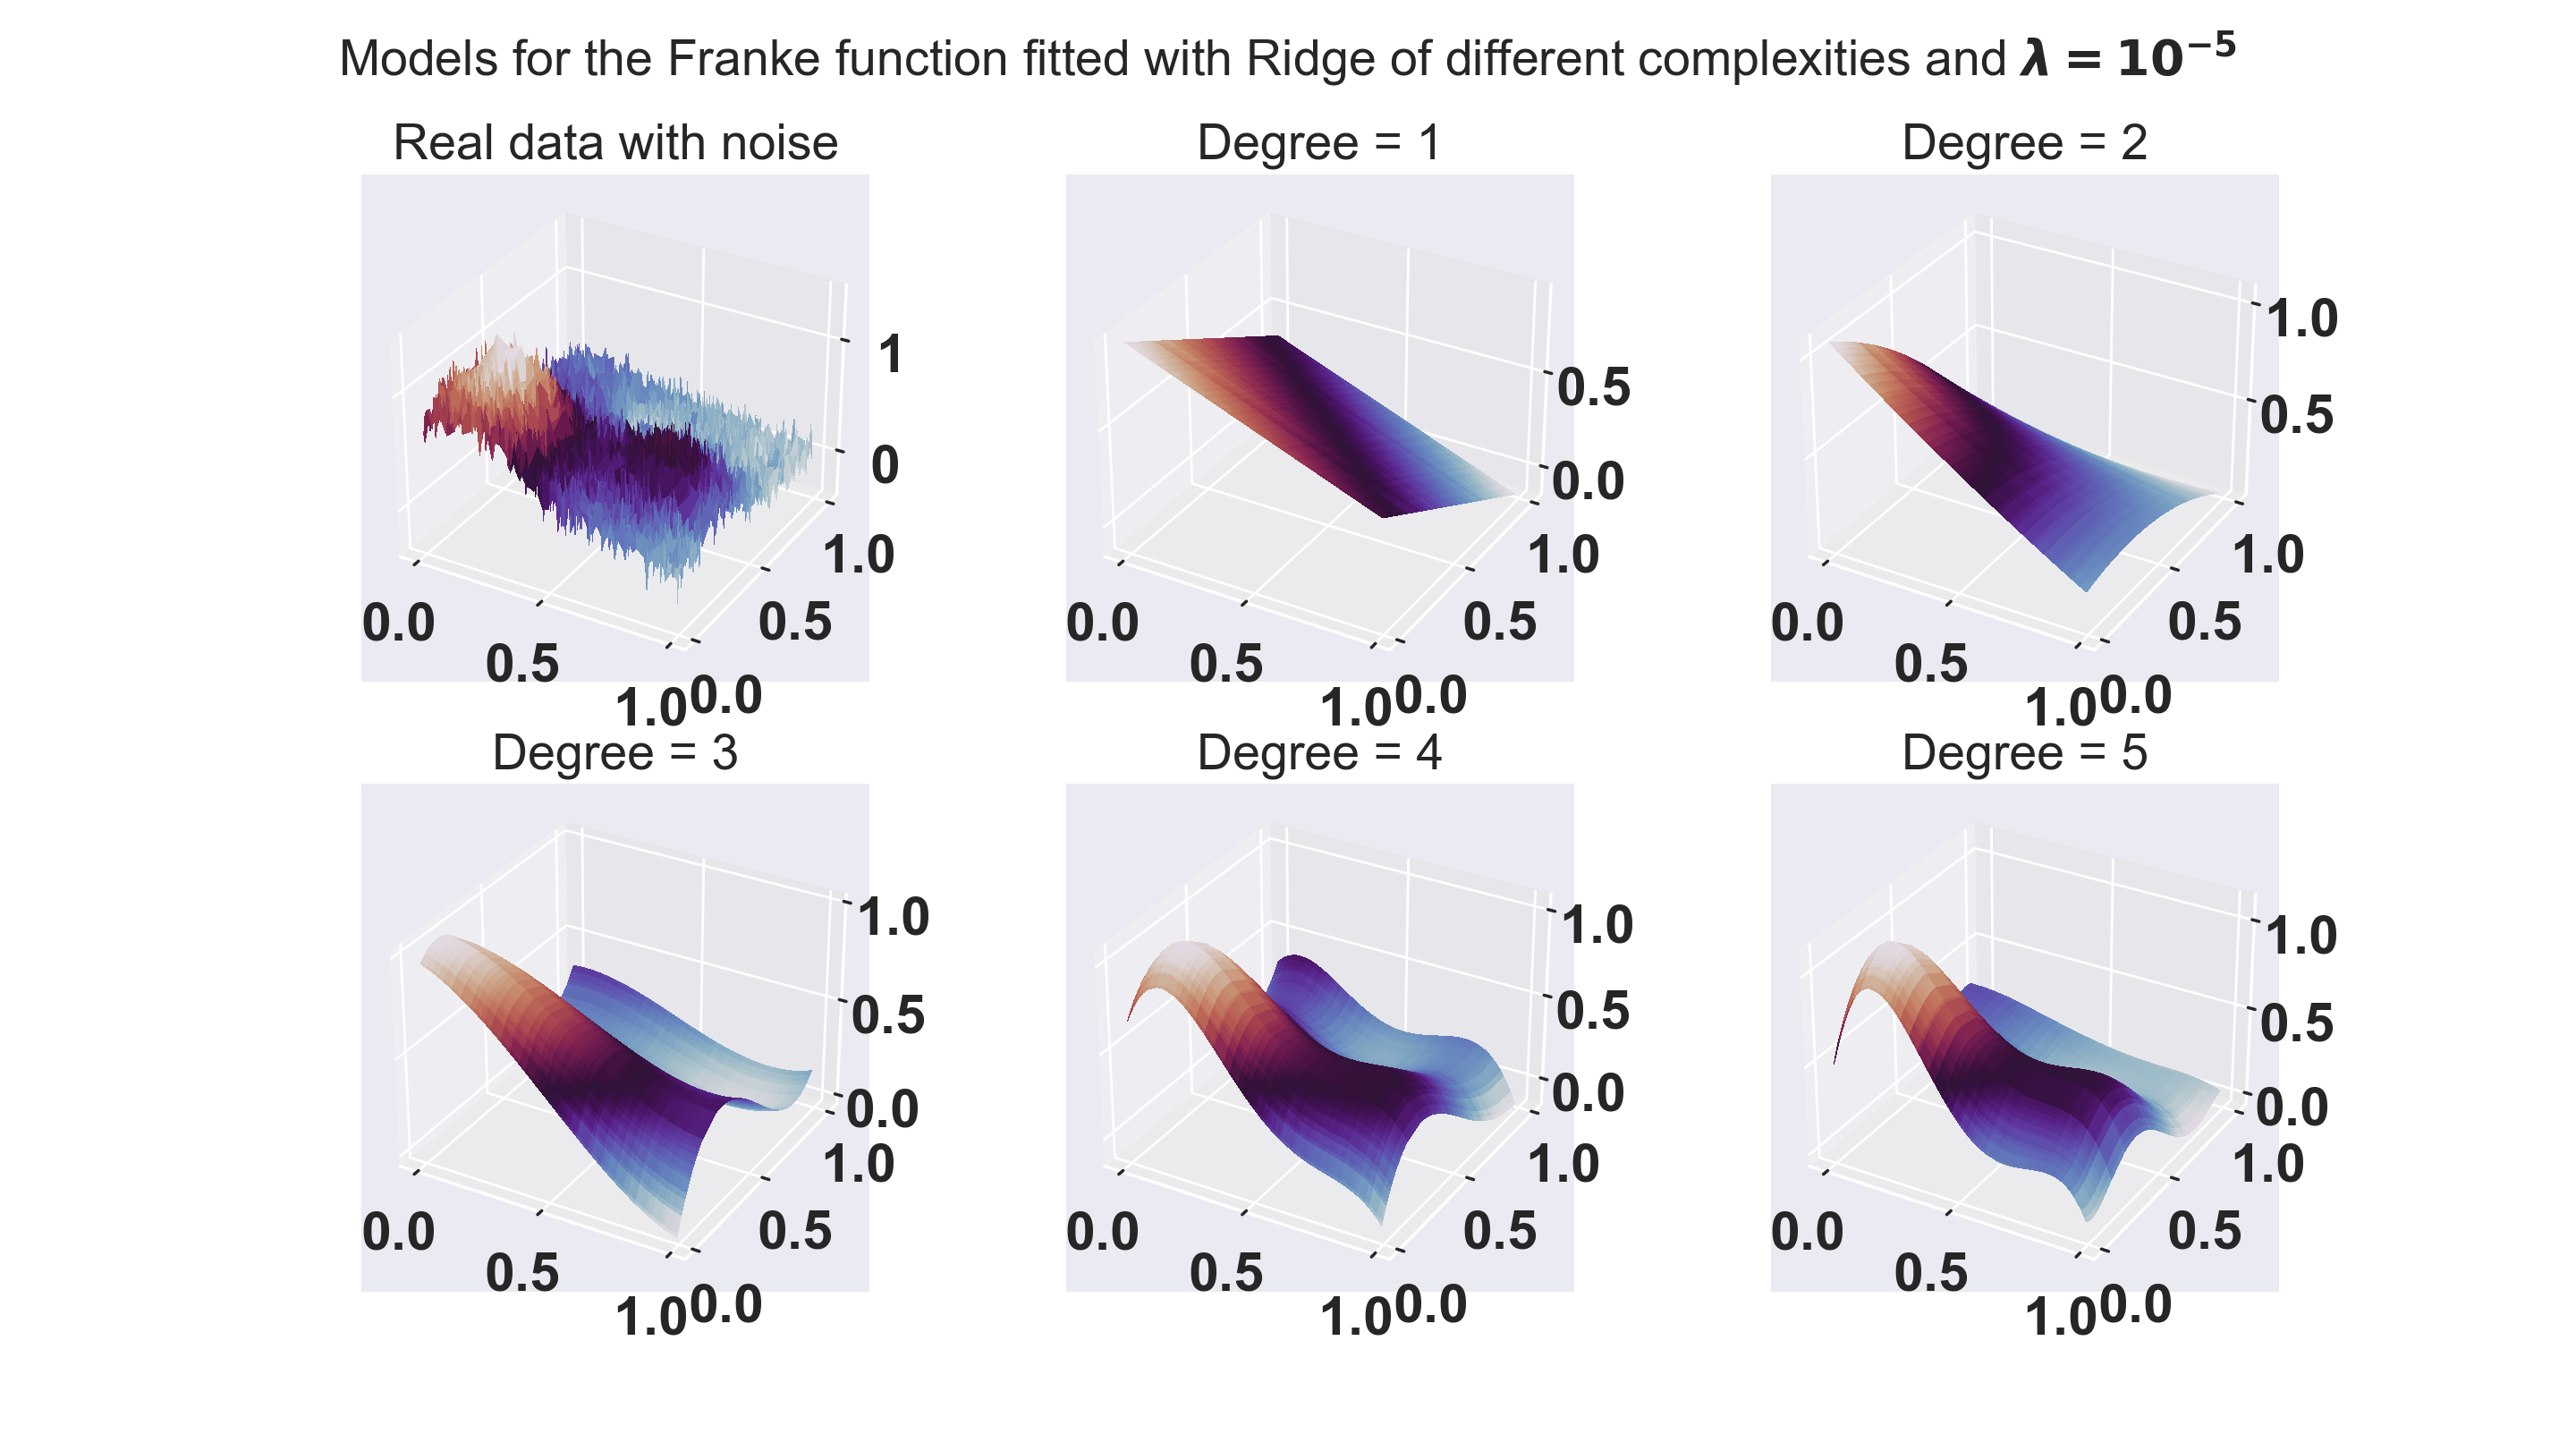
\includegraphics[width=\linewidth]{images/Figure_6.png}
	\caption{}
	\label{Ridge figure}
\end{figure}

\subsection{Terrain data}
\begin{figure}[H]
	\centering
	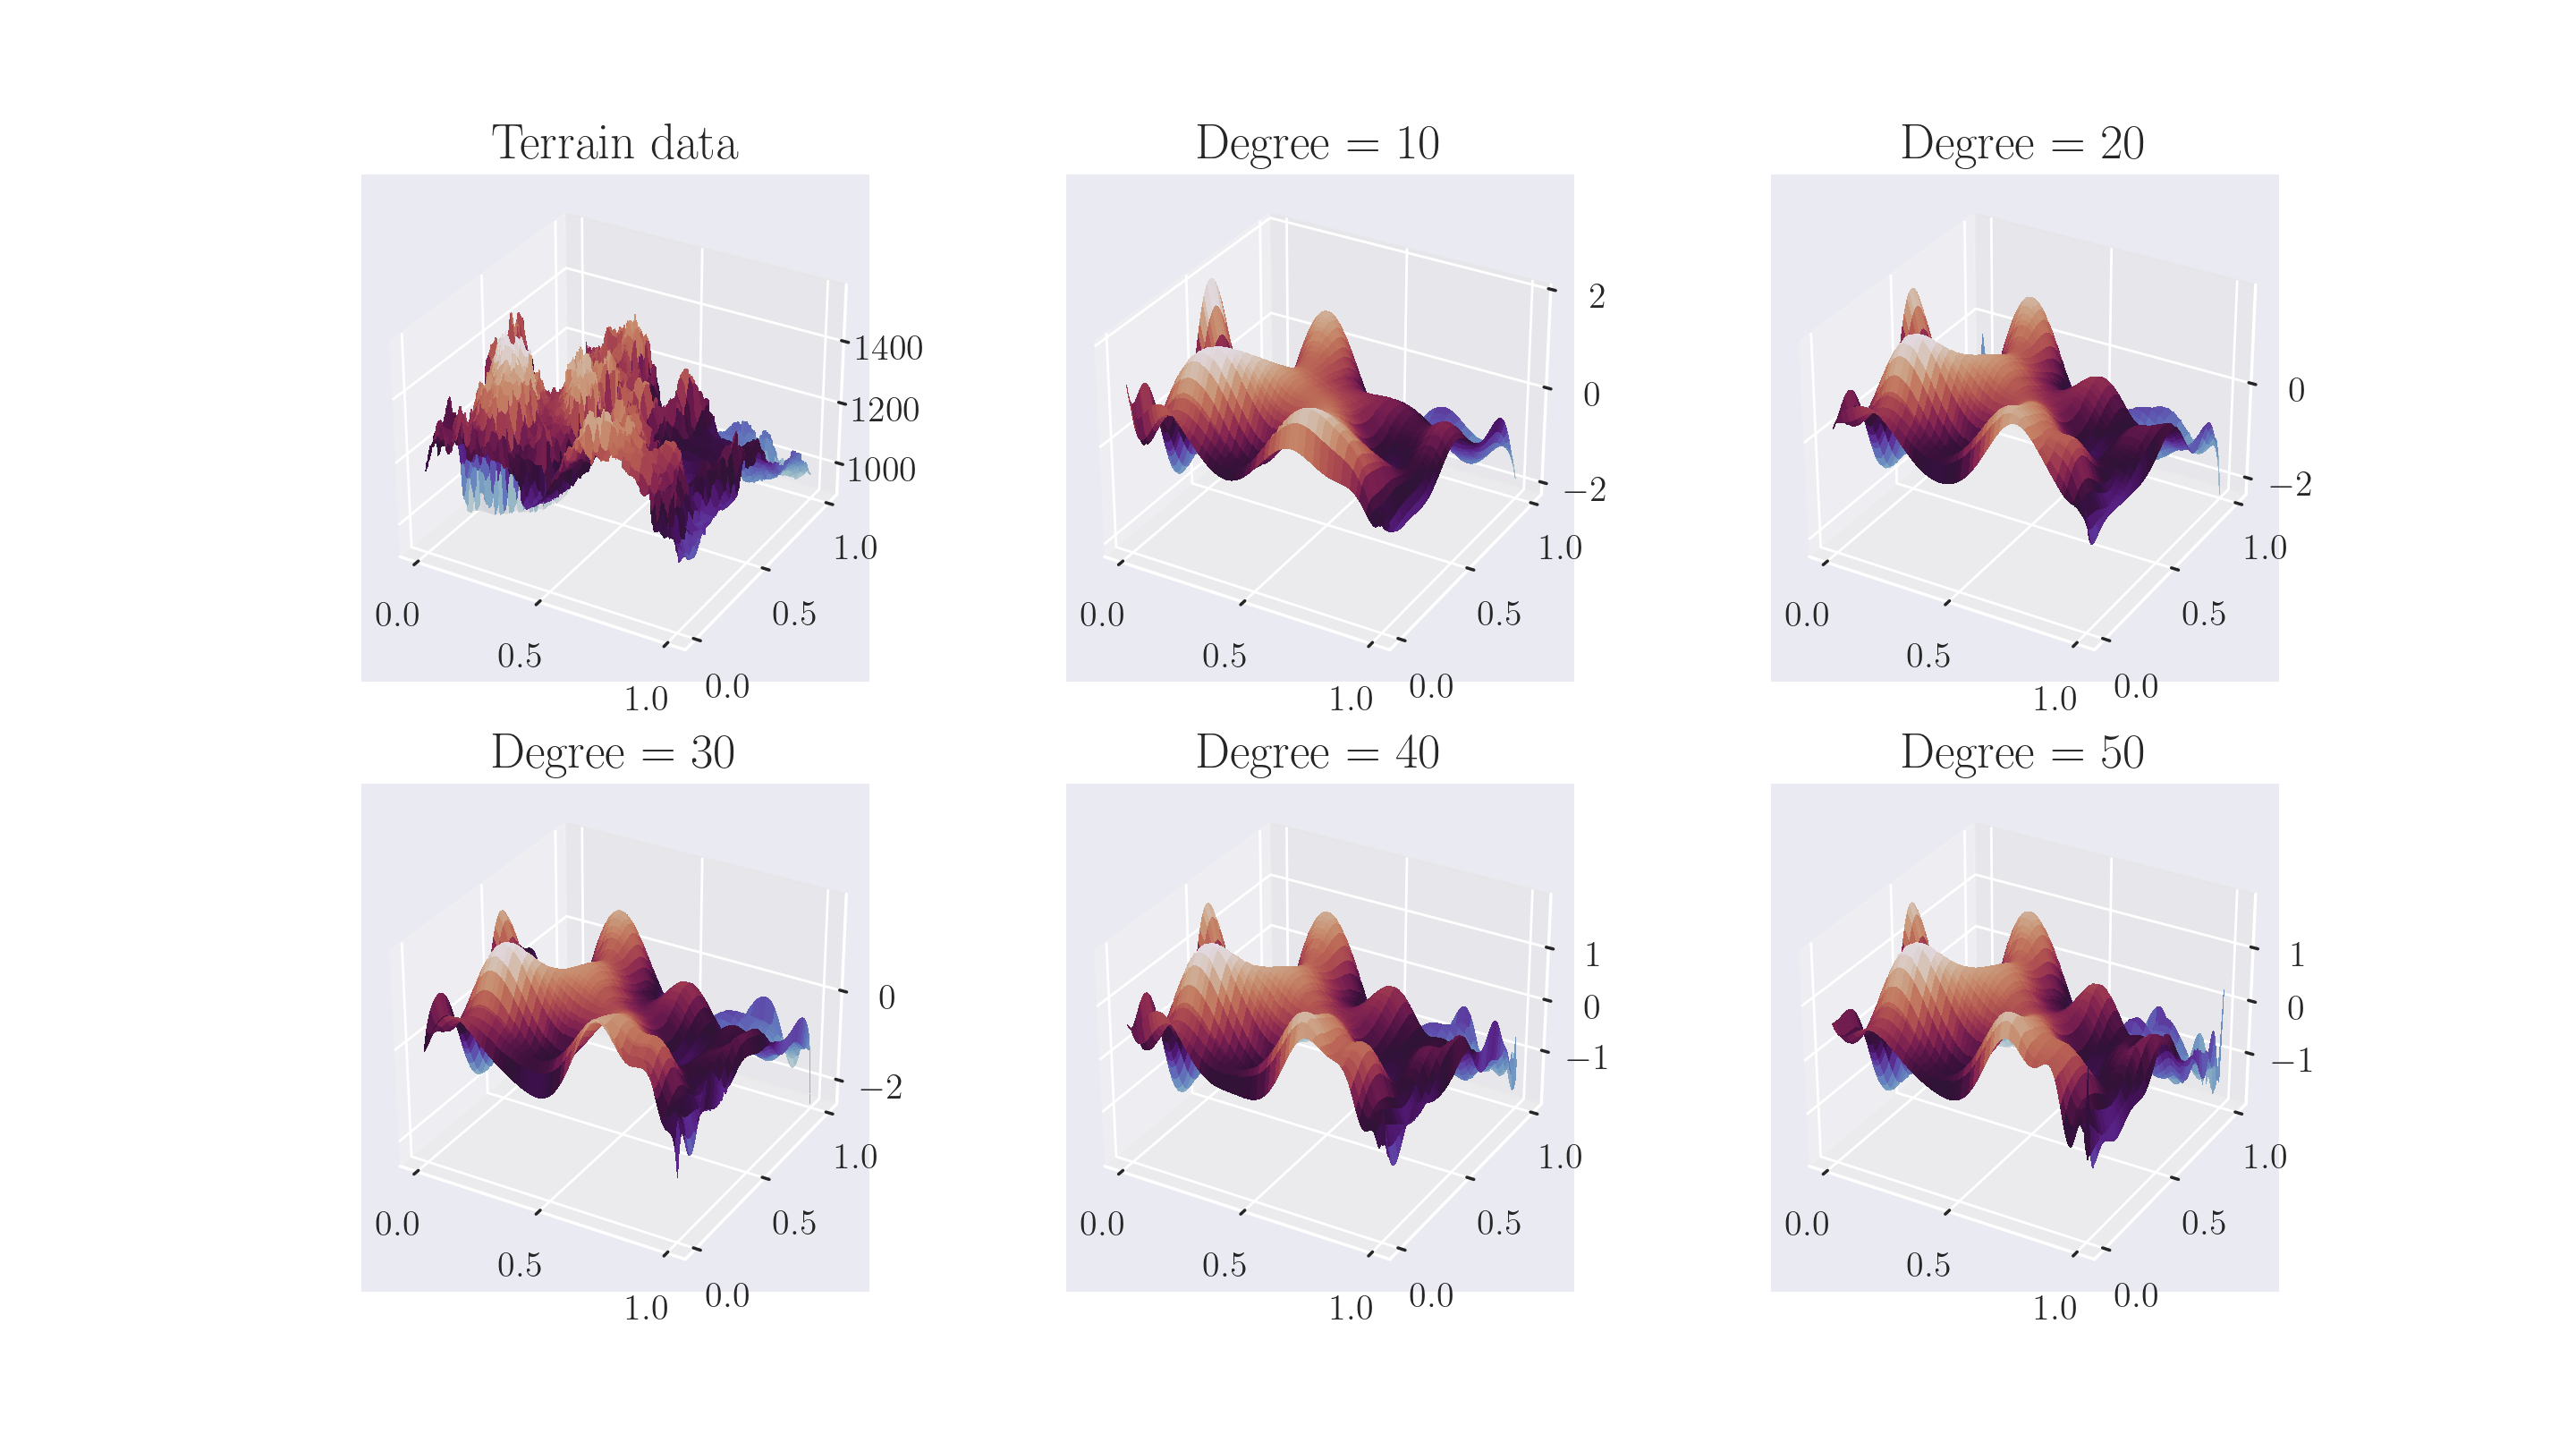
\includegraphics[width=\linewidth]{images/Figure_30.png}
	\caption{A 3D plot of the terrain data compared to models created with OLS of complexity 10, 20, 30, 40 and 50}
	\label{OLS 3D figure terrain data}
\end{figure}
%
\begin{figure}[H]
	\centering
	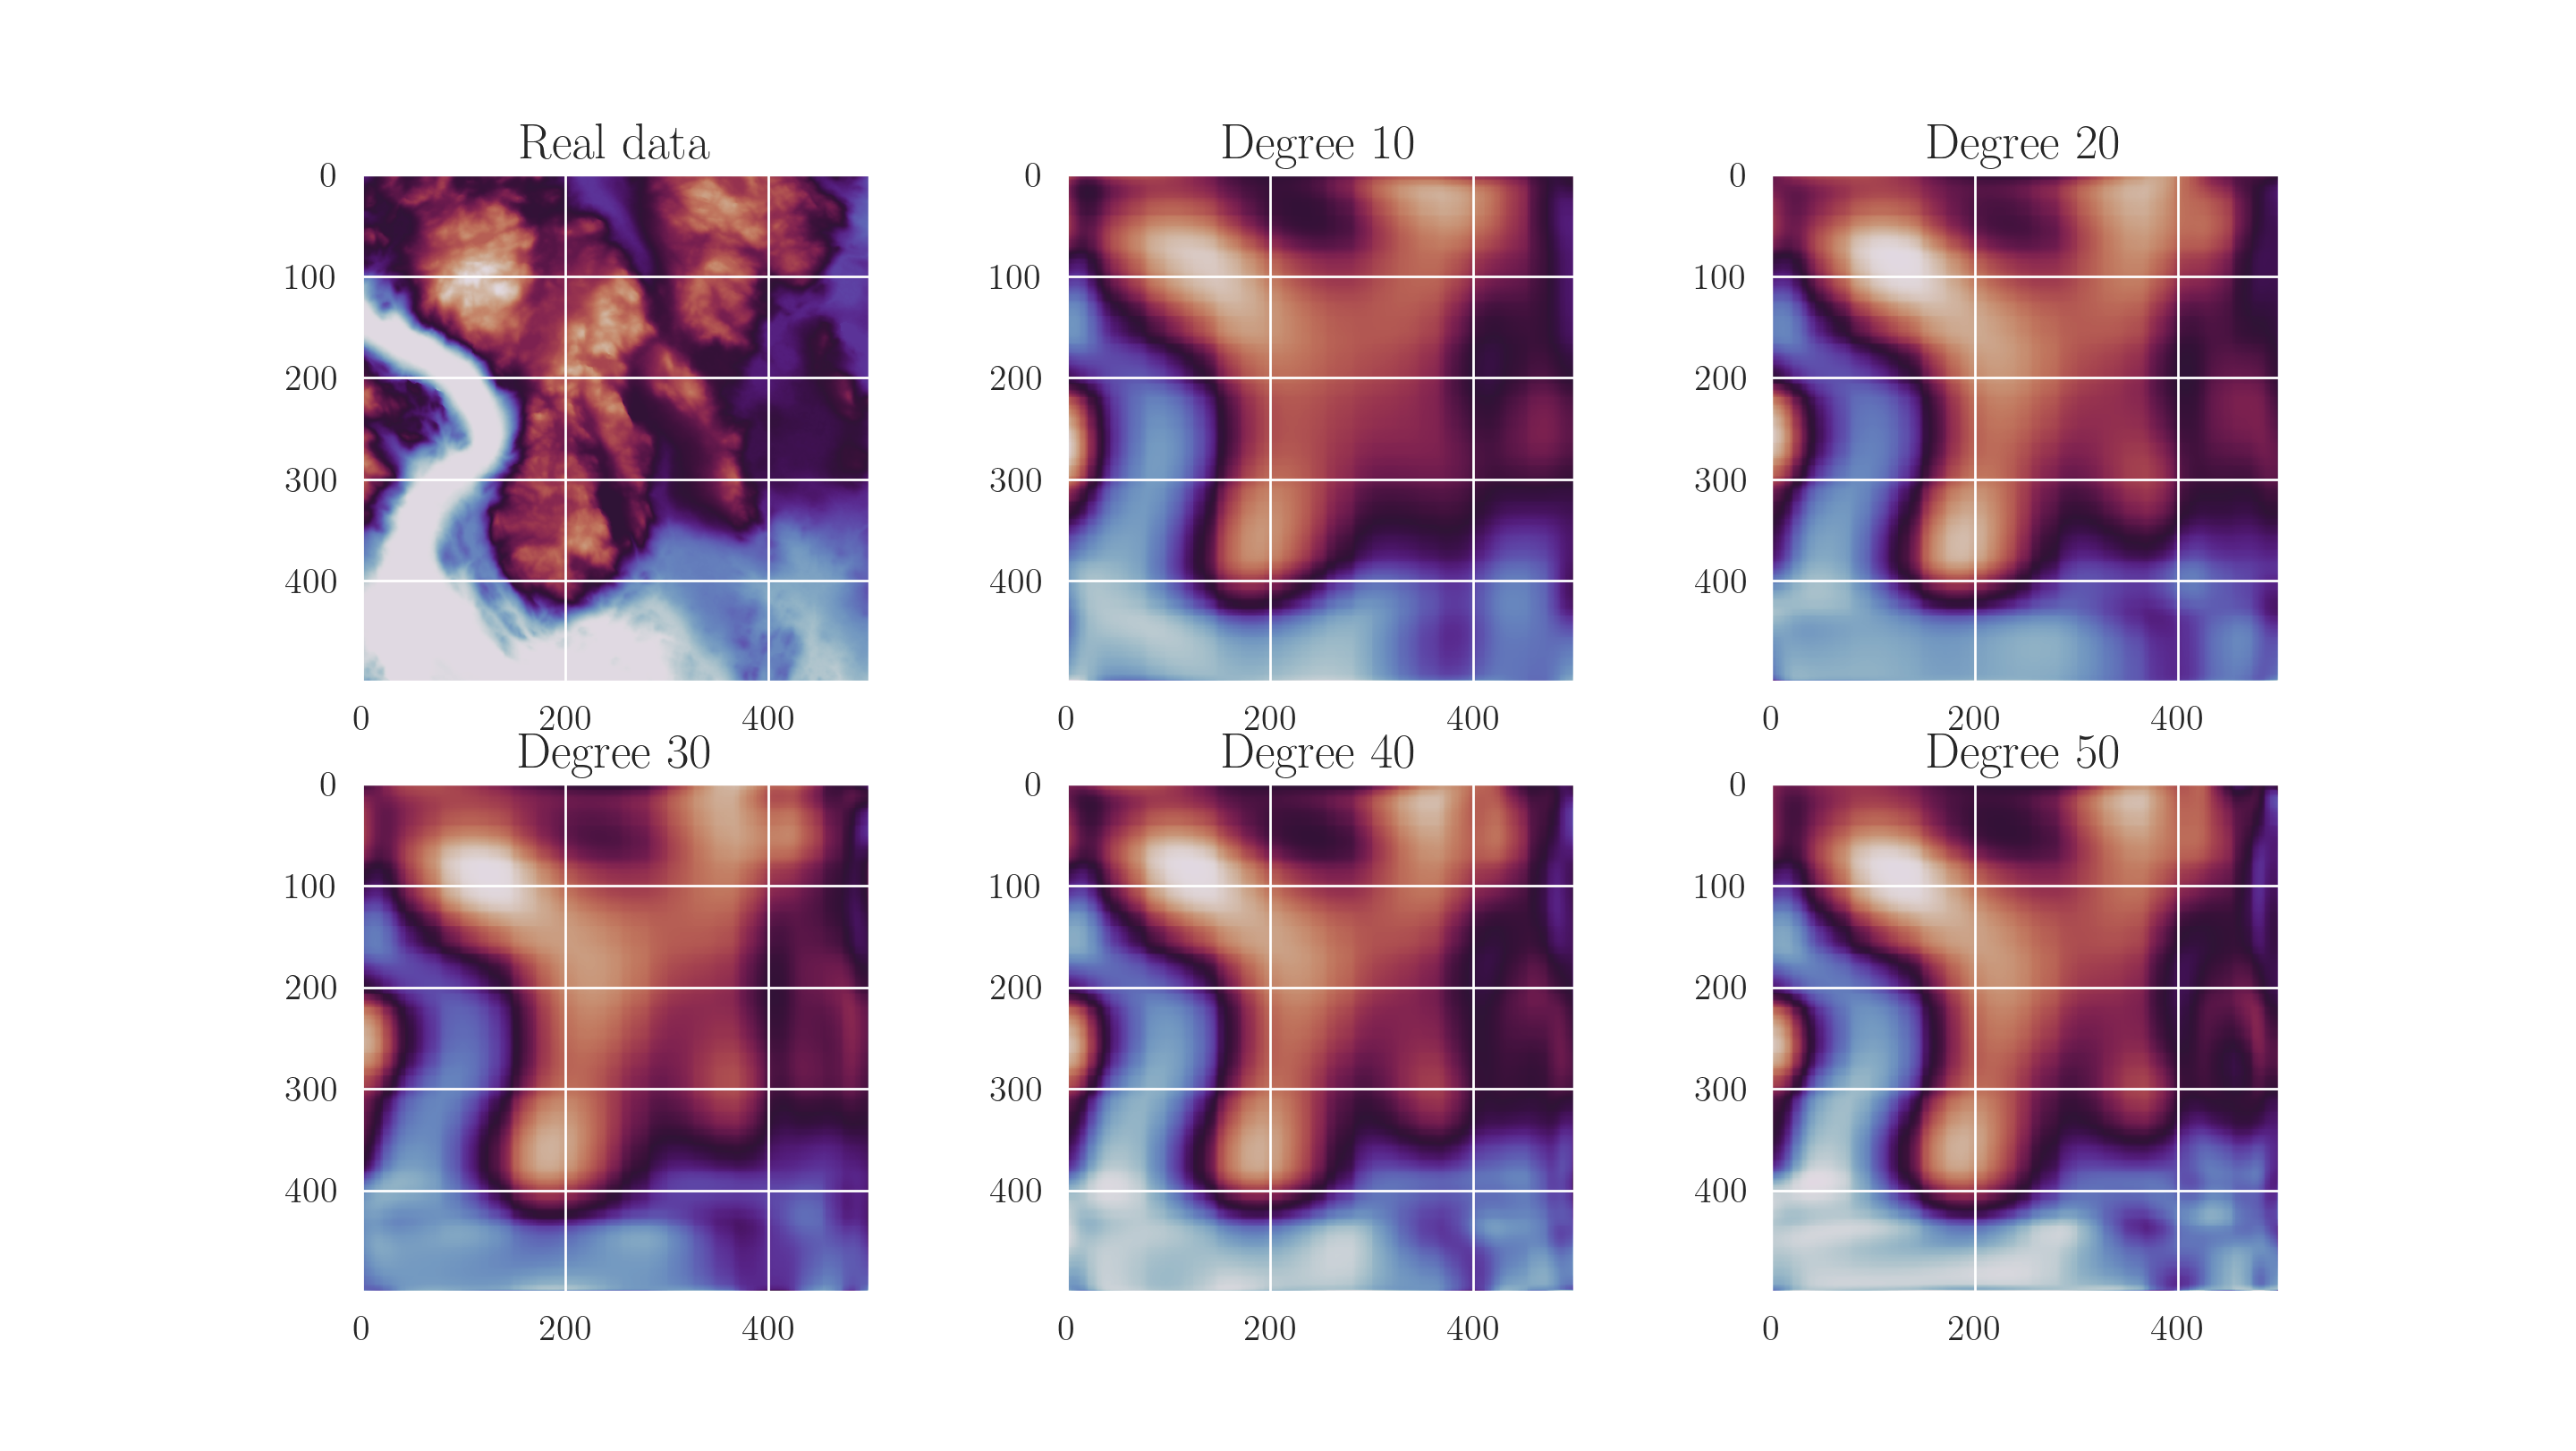
\includegraphics[width=\linewidth]{images/Figure_31.png}
	\caption{A 2D plot of the terrain data compered to models created with OLS of complexity 10, 20, 30, 40 and 50}
	\label{OLS 2D figure terrain data}
\end{figure}
%
\begin{figure}[H]
	\centering
	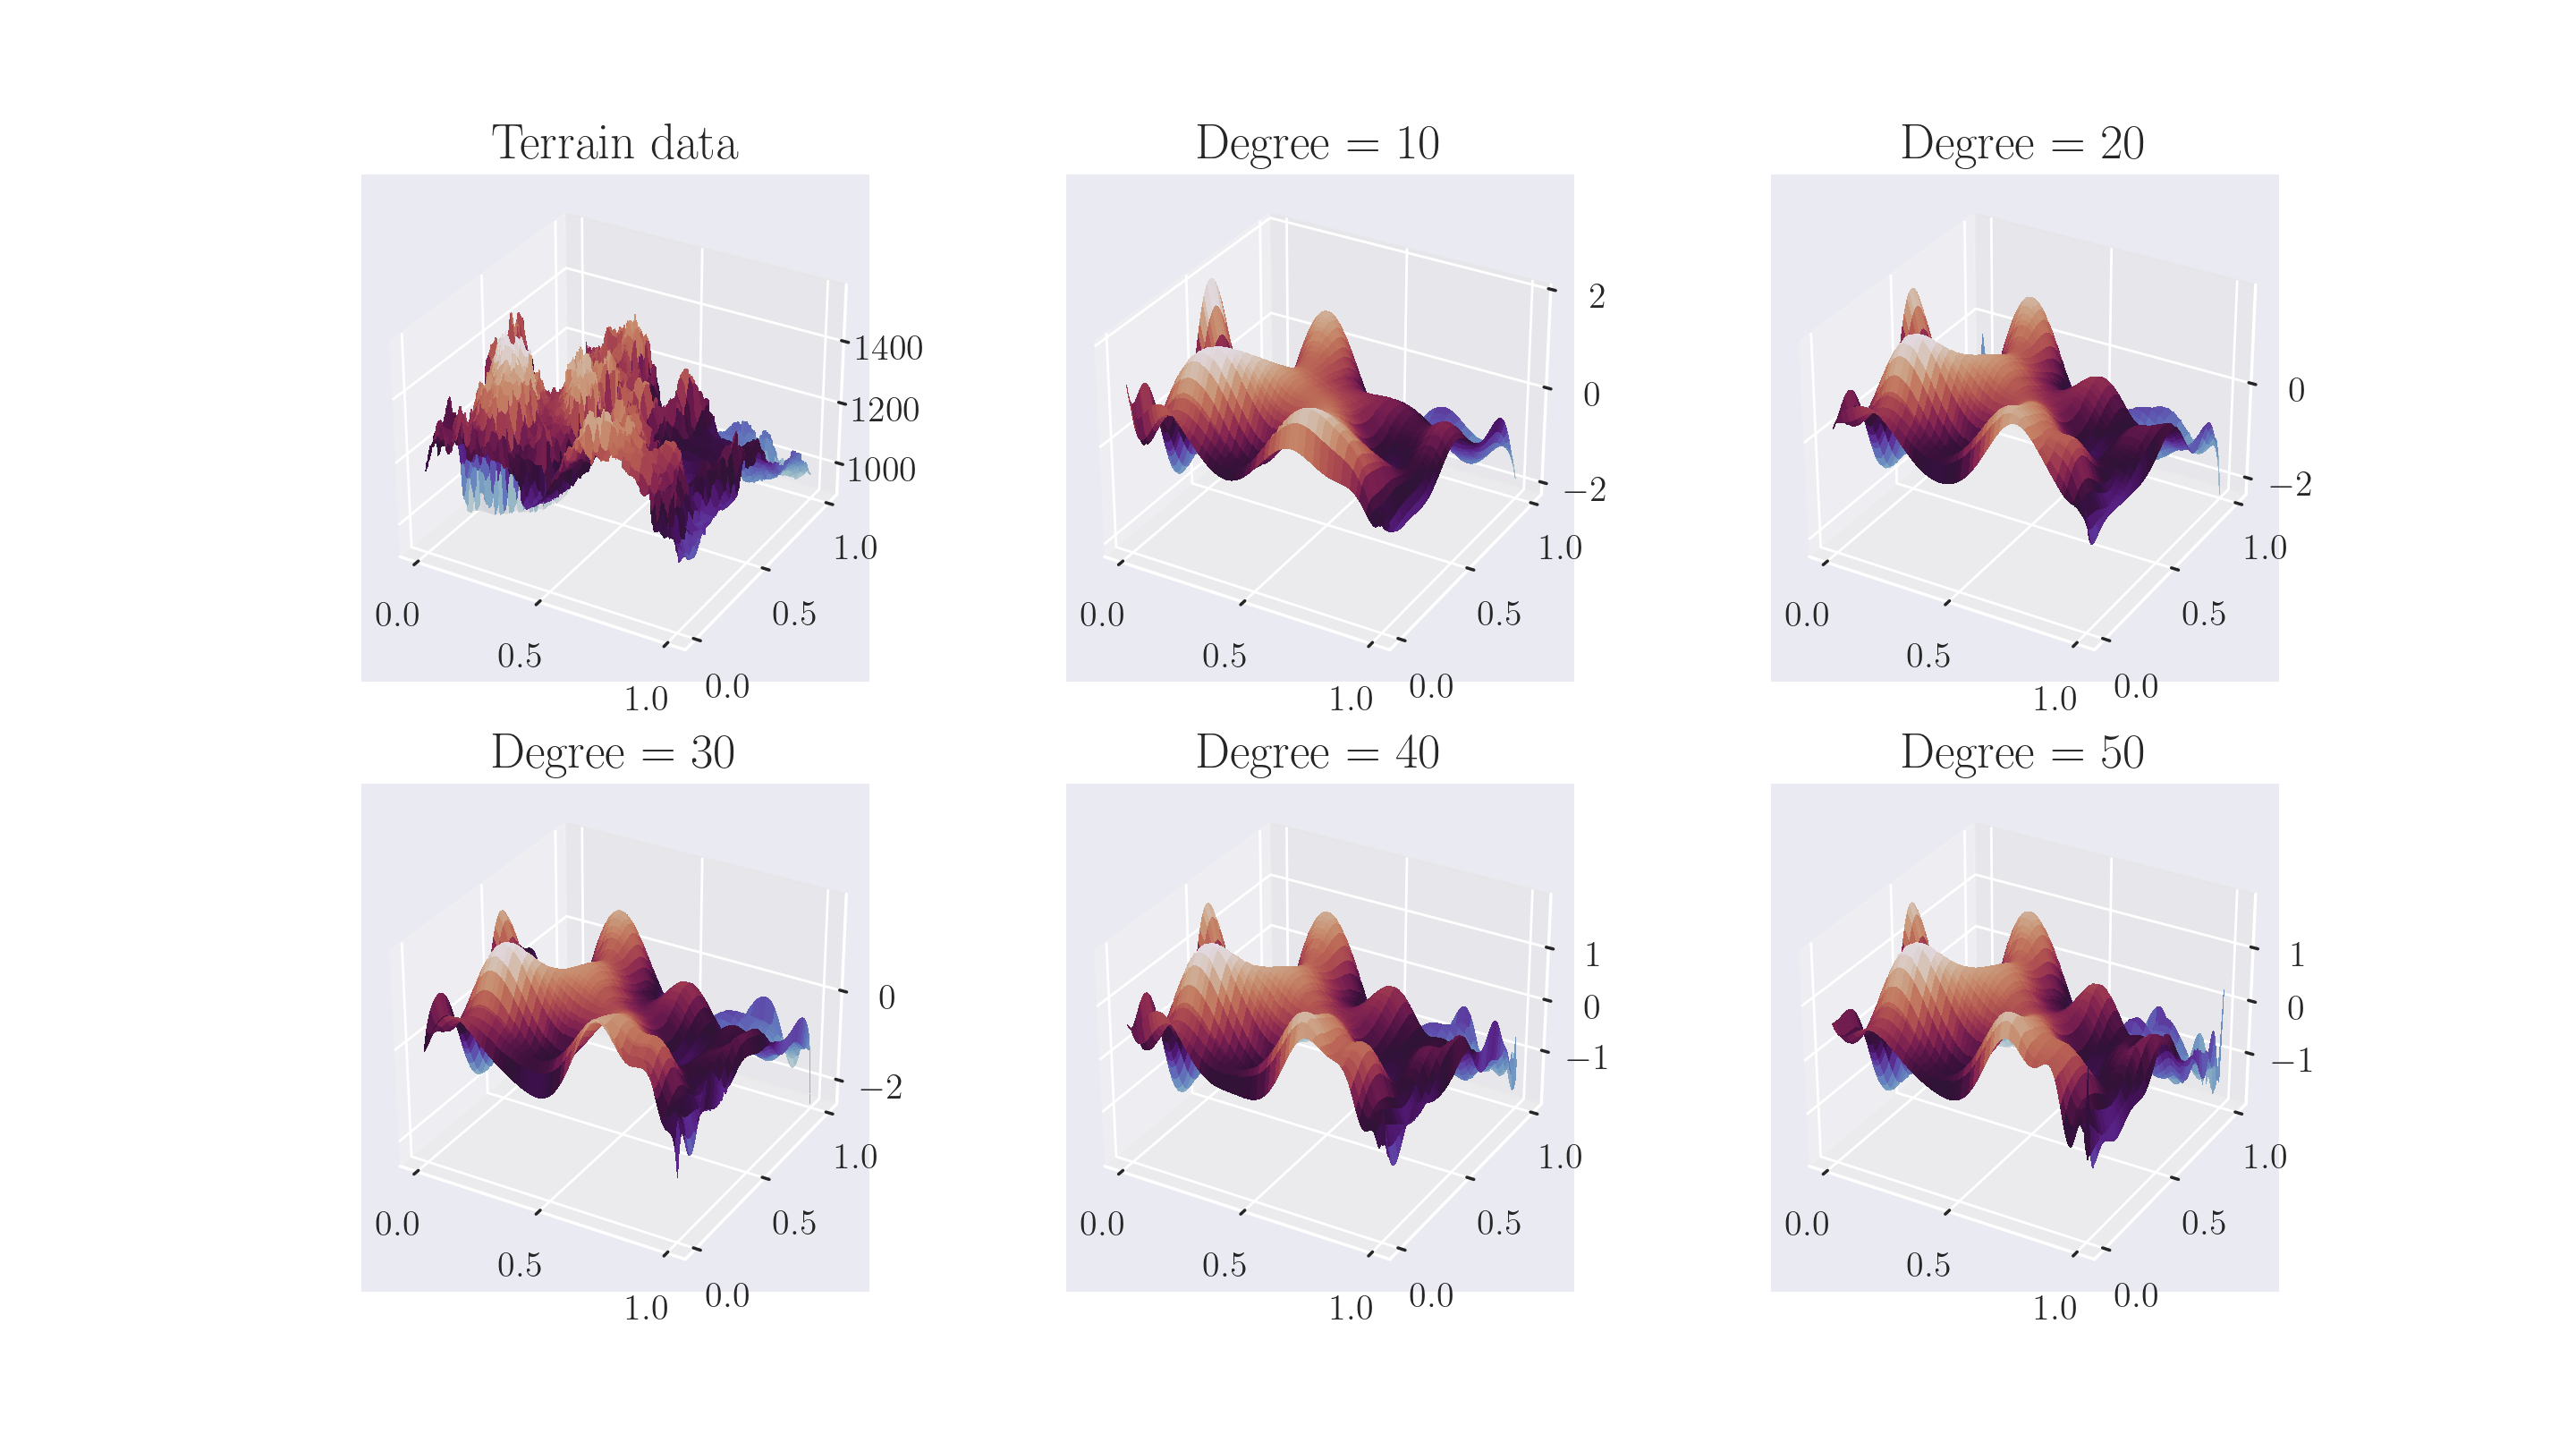
\includegraphics[width=\linewidth]{images/Figure_30.png}
	\caption{A 3D plot of the terrain data compered to models created with Ridge of complexity 10, 20, 30, 40 and 50 and a $\lambda$ value of $10^{-5}$}
	\label{Ridge 3D figure terrain data}
\end{figure}
%
\begin{figure}[H]
	\centering
	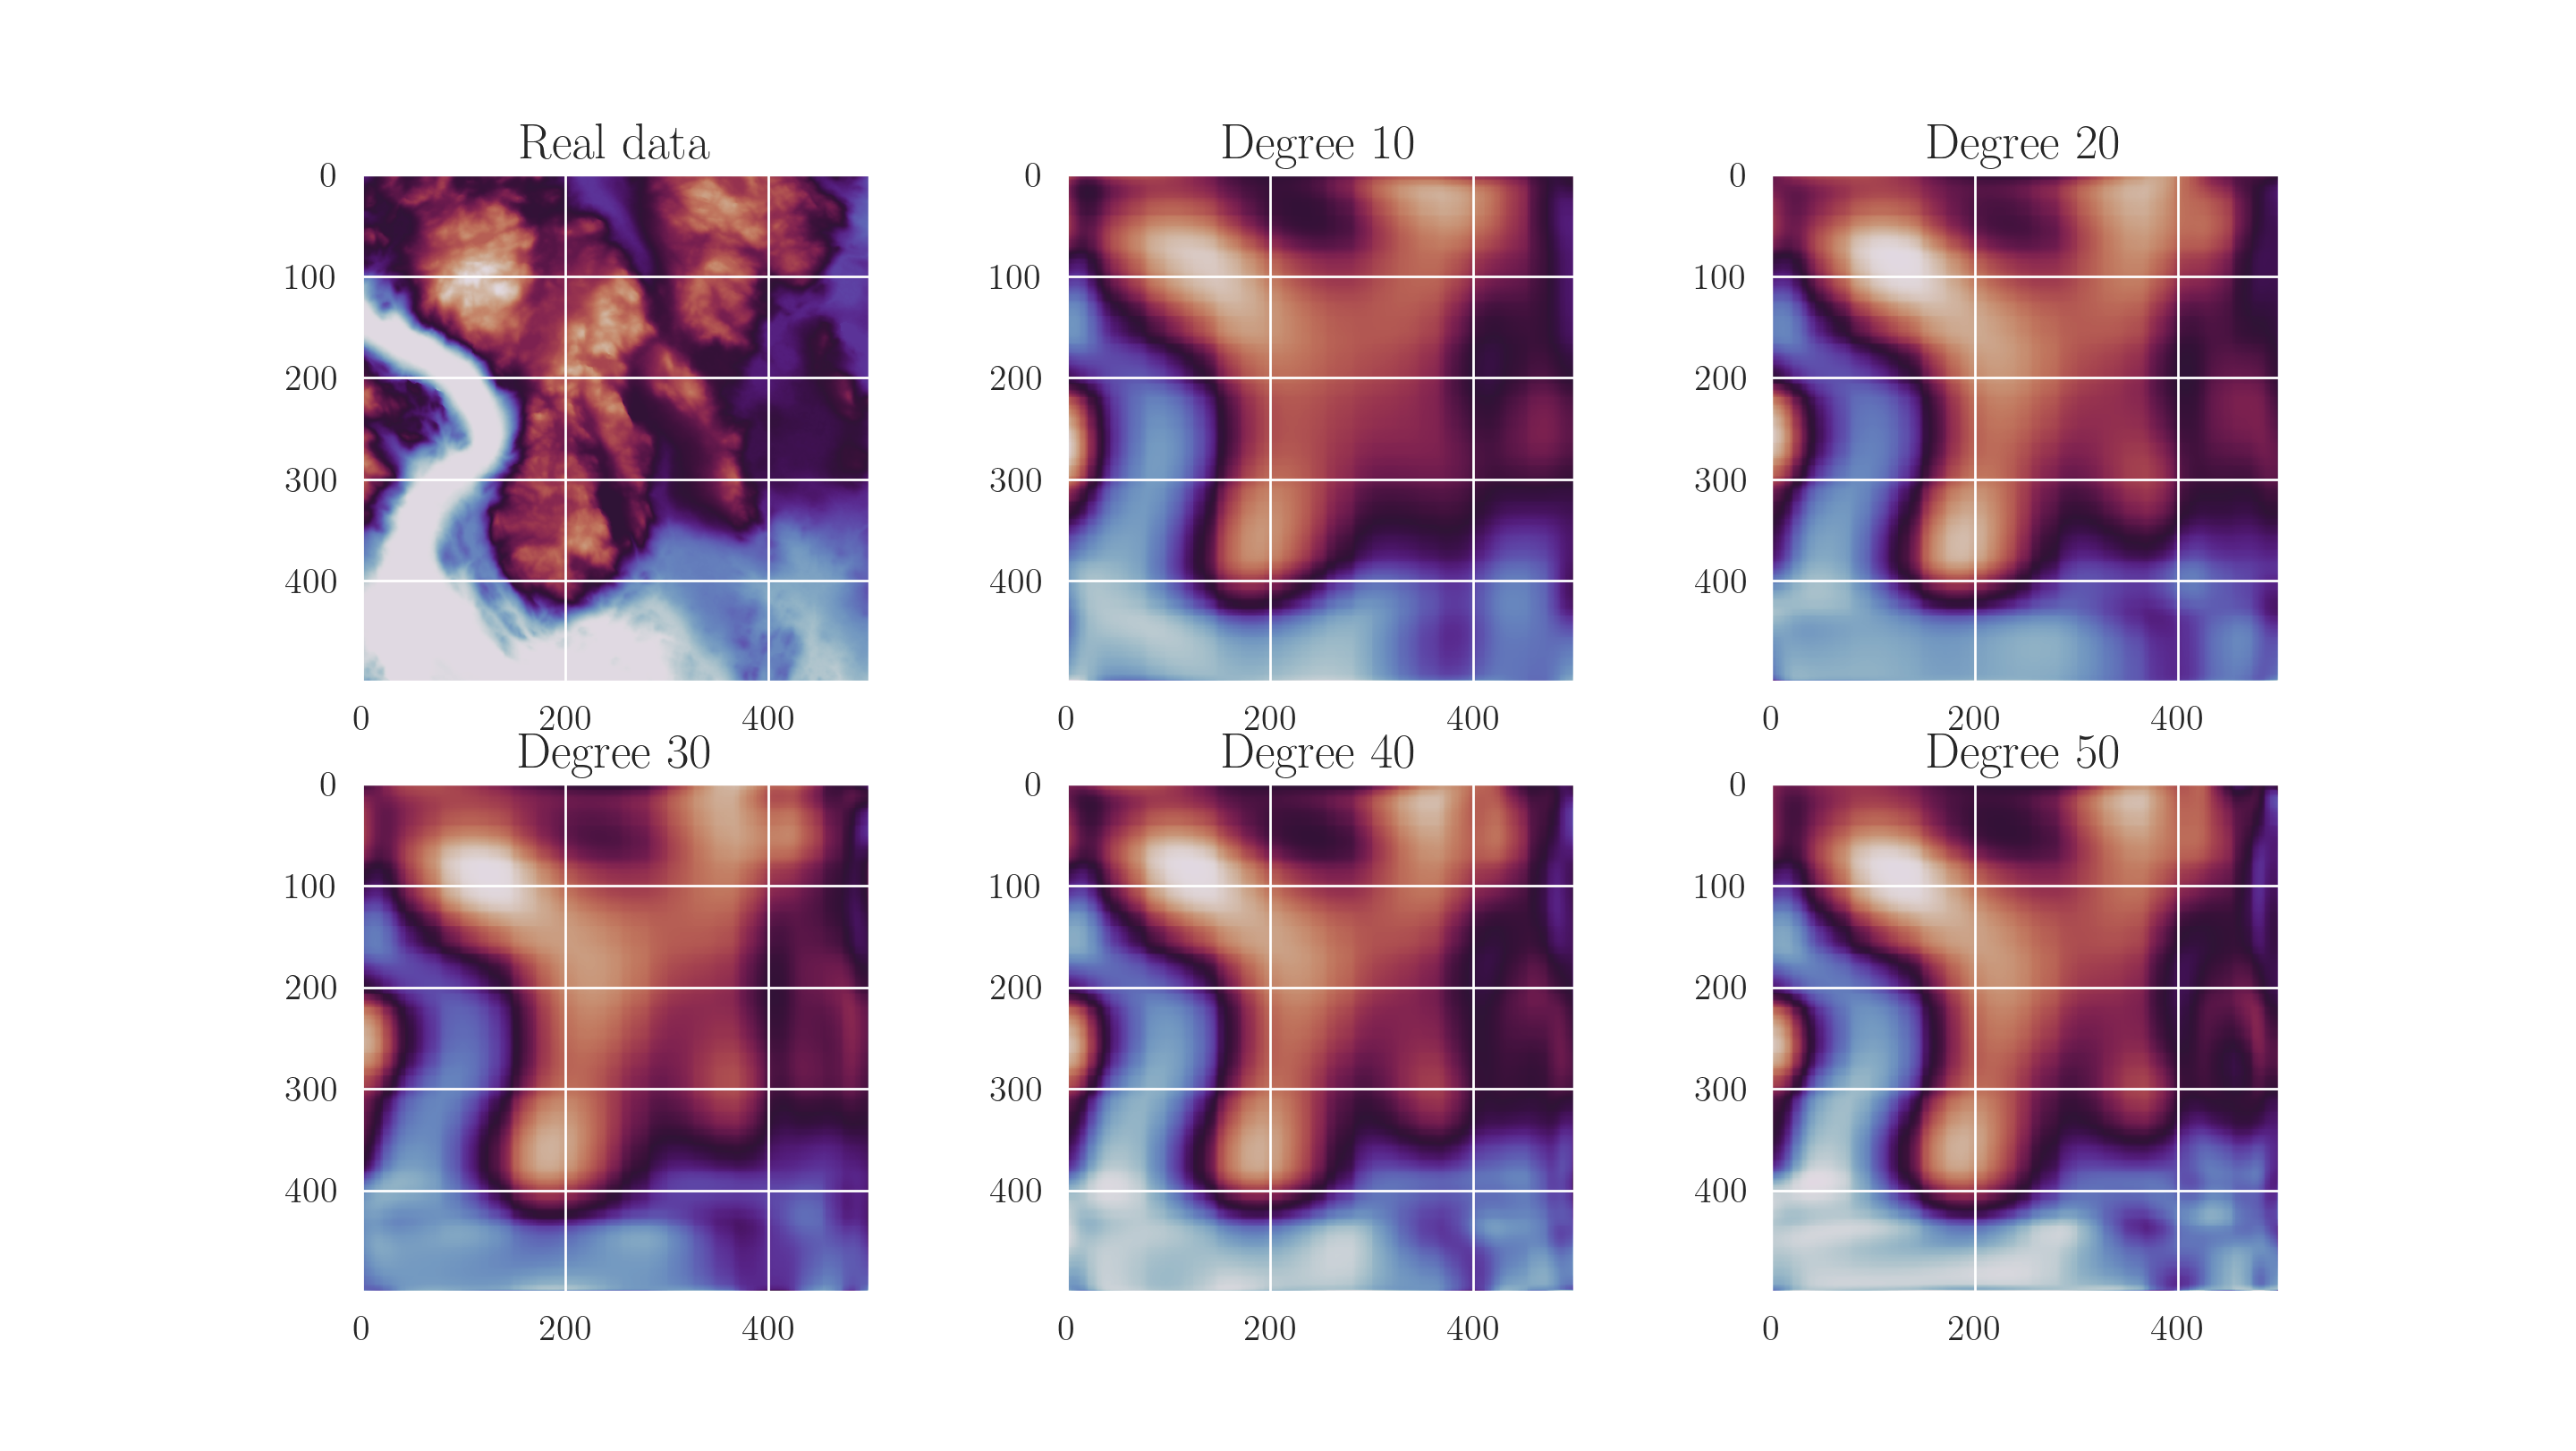
\includegraphics[width=\linewidth]{images/Figure_31.png}
	\caption{A 2D plot of the terrain data compered to models created with Ridge of complexity 10, 20, 30, 40 and 50 and a $\lambda$ value of $10^{-5}$}
	\label{Ridge 2D figure terrain data}
\end{figure}